\documentclass[12pt]{article}
\usepackage[margin=1in]{geometry}
\usepackage{amsmath}
\usepackage{amssymb}
\usepackage{tikz}
\usepackage{pgfplots}
\usepackage{eso-pic}
\pgfplotsset{compat=1.18}

\AddToShipoutPictureBG{%
  \begin{tikzpicture}[remember picture,overlay]
    \foreach \y in {0,1,...,27} {
      \draw[gray!20, very thin] 
        ([yshift=-\y cm]current page.north west) -- 
        ([yshift=-\y cm]current page.north east);
    }
  \end{tikzpicture}
}

\setlength{\parindent}{0pt}
\setlength{\parskip}{8pt}

\title{Week 8: Review of Weeks 1--7}
\author{
	Student: SA\\
	Tutor: Rachel Eglash}
\date{November 1, 2025}

\begin{document}
	
	\maketitle

	\section*{Session 8.2 Homework}
        
        \textbf{Instructions:} Show all work. Circle your final answers.
        
        \subsection*{Topics Covered:}
        \begin{itemize}
            \item Week 2: Solving Linear Equations
            \item Week 3: Inequalities (Absolute Value)
            \item Week 5: Systems of Linear Equations
            \item Week 6: Linear Functions \& Lines (Parallel/Perpendicular)
            \item Week 7: Systems Applications \& Inequalities
        \end{itemize}
	    
        \newpage
	
	    \subsection*{Quick Reference: Key Formulas \& Concepts}
	
	        \subsubsection*{Absolute Value Inequalities}
		    	For $|x| < a$ (where $a > 0$): $-a < x < a$ \\
                For $|x| > a$ (where $a > 0$): $x < -a$ OR $x > a$
	
	        \subsubsection*{Parallel \& Perpendicular Lines}
			    \textbf{Parallel lines:} Same slope $(m_1 = m_2)$ \\
                \textbf{Perpendicular lines:} Negative reciprocal slopes $(m_1 \cdot m_2 = -1)$
	
	        \subsubsection*{Systems of Equations}
	    		\textbf{One solution:} Lines intersect (different slopes) \\
                \textbf{No solutions:} Lines are parallel (same slope, different intercepts) \\
                \textbf{Infinitely many solutions:} Same line

            \subsubsection*{Distance Formula (Motion)}
                $d = rt$ \quad (distance = rate $\times$ time)

            \subsubsection*{Mixture Problems}
                (concentration$_1$)(volume$_1$) + (concentration$_2$)(volume$_2$) = (concentration$_{\text{final}}$)(volume$_{\text{final}}$)

            \newpage
	
        \section*{Part A: Equations \& Special Cases}

            \textbf{Problem 1}\\\\
            Solve: $3(x - 4) = 3(x + 7)$

            \vspace{4cm}

            \textbf{Problem 2}\\\\
            Solve: $2(x + 5) - 3 = 2x + 7$

            \vspace{4cm}

            \textbf{Problem 3}\\\\
            Solve: $\displaystyle\frac{x}{4} + 5 = \frac{x}{3} + 2$

            \newpage

        \section*{Part B: Absolute Value Inequalities}

            \textbf{Problem 4}\\\\
            Solve: $|x + 2| < 6$

            \vspace{3cm}

            \textbf{(a)} Graph the solution on a number line.

            \vspace{0.5cm}

            \begin{center}
            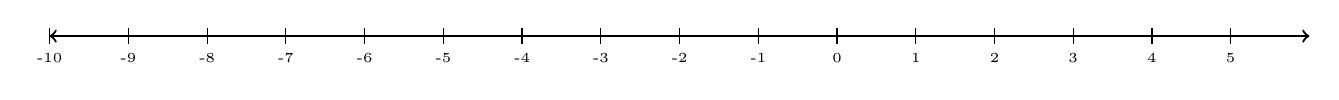
\begin{tikzpicture}
                \draw[<->,thick] (-10,0) -- (6,0);
                \foreach \x in {-10,-9,-8,-7,-6,-5,-4,-3,-2,-1,0,1,2,3,4,5}
                    \draw (\x,0.1) -- (\x,-0.1) node[below] {\tiny\x};
            \end{tikzpicture}
            \end{center}

            \vspace{0.5cm}

            \textbf{(b)} Write the solution in interval notation.

            \vspace{2cm}

            \textbf{Problem 5}\\\\
            Solve: $|3x - 1| \geq 8$

            \vspace{3cm}

            \textbf{(a)} Graph the solution on a number line.

            \vspace{0.5cm}

            \begin{center}
            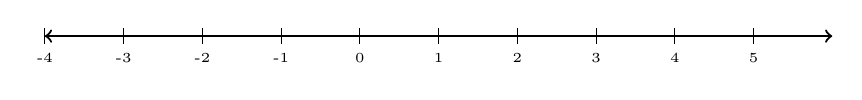
\begin{tikzpicture}
                \draw[<->,thick] (-4,0) -- (6,0);
                \foreach \x in {-4,-3,-2,-1,0,1,2,3,4,5}
                    \draw (\x,0.1) -- (\x,-0.1) node[below] {\tiny\x};
            \end{tikzpicture}
            \end{center}

            \vspace{0.5cm}

            \textbf{(b)} Write the solution in interval notation.

            \newpage

            \textbf{Problem 6}\\\\
            A machine part must be 50 mm long.\\\\
            It is acceptable if the length differs by at most 0.8 mm.\\\\
            Let $L$ = measured length (in mm).

            \vspace{0.5cm}

            Write and solve an inequality for $L$.\\\\
            State the acceptable range.

            \vspace{3cm}

            \textbf{(a)} Graph the solution on a number line.

            \vspace{0.5cm}

            \begin{center}
            \begin{tikzpicture}
                \draw[<->,thick] (46,0) -- (54,0);
                \foreach \x in {46,47,48,49,50,51,52,53,54}
                    \draw (\x-46,0.1) -- (\x-46,-0.1) node[below] {\tiny\x};
            \end{tikzpicture}
            \end{center}

            \vspace{0.5cm}

            \textbf{(b)} Write the solution in interval notation.

            \newpage

        \section*{Part C: Parallel \& Perpendicular Lines}

            \textbf{Problem 7}\\\\
            Find the equation of the line through $(-3, 2)$ and parallel to $y = -3x + 5$

            \vspace{4cm}

            \textbf{Problem 8}\\\\
            Find the equation of the line through $(4, 1)$ and perpendicular to $3x - y = 9$

            \vspace{4cm}

            \textbf{Problem 9}\\\\
            Determine if the lines are parallel, perpendicular, or neither:

            \begin{itemize}
                \item Line 1: $y = \displaystyle\frac{2}{5}x + 3$
                \item Line 2: $y = -\displaystyle\frac{5}{2}x - 1$
            \end{itemize}

            \newpage

        \section*{Part D: Systems of Linear Equations}

            \textbf{Problem 10}\\\\
            Solve the system using substitution:
            \begin{align*}
                y &= 2x - 5\\
                y &= -x + 7
            \end{align*}

            \vspace{4cm}

            \textbf{Problem 11}\\\\
            Solve the system using elimination:
            \begin{align*}
                4x + 3y &= 10\\
                -4x + 5y &= 6
            \end{align*}

            \vspace{4cm}

            \textbf{Problem 12}\\\\
            Classify the system (one solution / no solutions / infinitely many solutions):
            \begin{align*}
                y &= \frac{1}{2}x + 4\\
                2y &= x + 8
            \end{align*}

            \newpage

        \section*{Part E: Systems Applications}

            \textbf{Problem 13: Motion Problem}\\\\
            Two trains leave the same station at the same time.\\\\
            They travel in opposite directions.\\\\
            Train A travels at 60 mph.\\\\
            Train B travels at 80 mph.\\\\
            After how many hours will they be 420 miles apart?

            \vspace{5cm}

            \textbf{Problem 14: Word Problem}\\\\
            A movie theater sold tickets for adults and children.\\\\
            There were 120 tickets sold in total.\\\\
            Each adult ticket cost \$15.\\\\
            Each child ticket cost \$8.\\\\
            The total revenue was \$1,470.\\\\
            How many of each type of ticket was sold?

\end{document}